\chapter{Anhang - Formale Fragen}
Die Formatierung der Vorlage ist beizubehalten. Die Farben in Diagrammen und Zeichnungen müssen so gewählt werden, dass durch das Ausdrucken der Arbeit in Schwarz-Weiß keine Informationen verloren gehen (Graustufen). Die Verwendung der Farbe gelb ist unzulässig. Weiterhin muss auf Personen mit einer Rotgrünblindheit bei der Farbwahl Rücksicht genommen werden. Die Zahlen von eins bis einschließlich zwölf werden ausgeschrieben. Höhere Zahlen werden \emph{nicht} ausgeschrieben. Diagramme, Tabelle, etc. sind so zu formatieren, dass sie inklusive ihrer Unterschriften bei einer Verkleinerung auf DIN A5 lesbar bleiben.
%
\section{Umgang mit Latex - Beispiele}
%
\minisec{Formeln}
Die Theorie beinhaltet Formeln, Herleitungen, empirische Daten, etc. Für die Darstellung von Formeln in der Formelumgebung bzw. im Fließtext gelten einige Regeln:

Das Multiplikationszeichen ist der Punkt und nicht der Stern. Verwendet wird er bei Skalarprodukten, oder wenn sonst Irrtümer entstehen können. Ansonsten macht ein Multipliaktionszeichen Formeln unübersichtlich lang. Um die Eindeutigkeit und Übersichtlichkeit in Formeln zu gewährleisten bietet es sich häufig an zusätzliche Abstandshalter und verschieden große Klammern zu verwenden. 
\begin{equation}
\begin{split}
%\dot{\gls{x}}&~=~\gls{A}\gls{x}(t)~+~%
%							  \gls{B}\gls{u}(t)\\
%\gls{y}&~=~\gls{C}\gls{x}(t)~+~\gls{D}\gls{u}(t)\\
\dot{\underline{x}}&~=~\underline{A}\underline{x}(t)~+~%
							  \underline{B}\underline{u}(t)\\
\underline{y}&~=~\underline{C}\underline{x}(t)~+~\underline{D}\underline{u}(t)\:.
\end{split}
\label{eq:Gleichung1}
\end{equation} \glsadd{A}\glsadd{B}\glsadd{C}\glsadd{D}\glsadd{x}\glsadd{u}
\begin{equation}
\begin{pmatrix} 		
	\delta\dot{q_k}		\\
	\delta\dot{\alpha_k}	\\
	\delta\dot{V_k}		\\
	\delta\dot{\gamma_k} \end{pmatrix}%
=\underbrace{\begin{bmatrix}	
	M_q			& M_{\alpha} 	& M_u 	& 0	\\ 
	1+Z_q 		& Z_{\alpha} 	& Z_u	& 0	\\
	X_q			& X_{\alpha}-g	& X_u 	& -g\\
	-Z_q 		& -Z_{\alpha} 	& -Z_u	& 0	\end{bmatrix}}_{\text{Zustandsmatrix}}%
\begin{pmatrix} 		
	\delta{q_k}			\\
	\delta{\alpha_k}	\\
	\delta{V_k}			\\
	\delta{\gamma_k} 	\end{pmatrix}%
+\underbrace{\begin{bmatrix}
	M_{F} 		& M_{\kappa}	& M_{\eta}\\
	Z_{F} 		& Z_{\kappa}	& Z_{\eta}\\
	X_{F} 		& X_{\kappa}	& X_{\eta}\\
	-Z_{F} 		& -Z_{\kappa}	& -Z_{\eta}\end{bmatrix}}_{\text{Eingangsmatrix}}%
\begin{pmatrix}
	\delta_F		\\
	\delta\kappa	\\
	\delta\eta 		\end{pmatrix}\:.
\label{eq:gleichung2}
\end{equation}
In der Formel-Umgebung wird Text so dargestellt, wie im Fließtext. Dazu verwendet man den Befehl $\backslash$text oder $\backslash$mathrm. Letzterer empfiehlt sich u.a. für Einheiten im Formeltext, da lediglich die Schriftart geändert wird, die Formel-Umgebung jedoch erhalten bleibt. Auch der Differentialoperator (Nicht zu verwechseln mit der partiellen Ableitung) bzw. Integrale werden nicht kursiv geschrieben:
\begin{equation}
E=\frac{\operatorname{d} \! \sigma}{\operatorname{d} \! \epsilon} \:.
\end{equation}
Partielle Ableitung:
\begin{equation}
\tau=G \;\left(\frac{\partial u}{\partial y} + \frac{\partial v}{\partial x}\right) \:.
\end{equation}

In abgesetzten Formeln werden Brüche mit horizontalem Bruchstrich (Befehl $\backslash$frac{}{}) verwendet  $\mathrm{\frac{N}{mm^2}}$. Im Fließtext werden Brüche mit einem Schrägstrich dargestellt. Dabei ist ausdrücklich die Formatierung \emph{ohne} Fraction-Umgebung, $\mathrm{N/mm^2}$, der Formatierung \emph{mit} einer Umgebung, wie dem Befehl $\backslash$sfrac{}{}, $\mathrm{\sfrac{N}{mm^2}}$, vorzuziehen.

Die Zeichen für die Dezimal- und Tausendertrennung richten sich nach der Sprache der Arbeit (vgl. Tabelle \ref{tab:Trennzeichen}). In Grafiken sollte man sich an die jeweiligen Konventionen halten, in deutschsprachigen Arbeiten ist es jedoch ebenso zulässig, die englische Konvention zu nutzen, sofern eine andere Darstellung nicht mit vertretbarem Aufwand erreichbar ist.
\begin{table}
\centering
\begin{tabular}{lrr}
\toprule
							& Deutsch	& Englisch\\
\midrule
Tausendertrennzeichen		& .			& ,\\
Dezimaltrennzeichen 		& ,			& .\\
\bottomrule
\end{tabular}
\caption{Dezimal- und Tausendertrennung, aufgeführt nach Sprachraum.}
\label{tab:Trennzeichen}
\end{table}
%
\minisec{Abbildungen}
Das Hinzufügen von Grafiken und Abbildungen dient der Veranschaulichung bzw. der Ergänzung des Fließtexts. Abbildungen werden mit der $\backslash$figure-Umgebung in den Text eingebunden. Der Befehl mit dem die jeweilige Abbildung aufgerufen wird lautet:\\
$\backslash$includegraphics[ scale=.71]\{pictures/Dateiname.eps\}. Dazu muss die verwendete Datei als .eps- bzw. als .png-Datei im Ordner \glqq pictures\grqq \! abgelegt werden. Mit Befehlen wie beispielsweise scale, angle, width, oder height in einer Latex-spezifischen Einheit wird das Bild bezüglich Skalierung, Drehwinkel, Breite oder Höhe angepasst. Bei Zeichnungen ist darauf zu achten, dass Zeichnungs- und Bemaßungslinien, sowie Schriftbreiten mit einem normgerechten Satz von Strichbreiten erstellt wurden. Bei Verwendung des Strichbreiten-Satzes [0,35mm; 0,7mm] ist in der Zeichnung eine Schriftgröße von 16pt in etwa normgerecht. Eine Skalierung dieser Zeichnung mit dem Faktor $\mathrm{=\:1/\sqrt{2}}$ ergibt einen Strichbreitensatz von [0,25mm; 0,5mm] und die entsprechende Schriftgröße von 12pt. Ein Beispiel ist in Abbildung \ref{fig:Bsp_Zeichung} dargestellt.
\begin{figure}[t!]
\centering
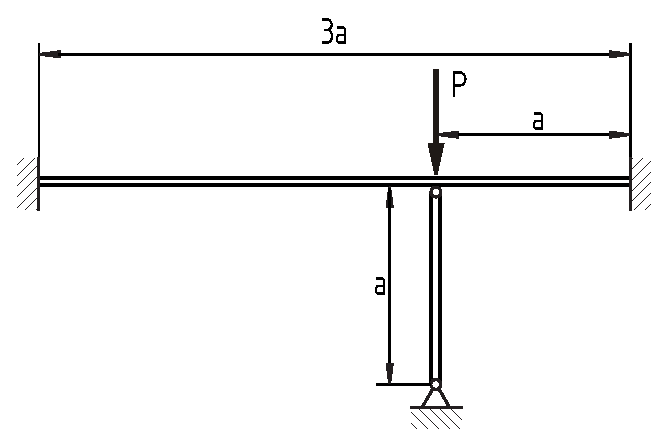
\includegraphics[scale=0.71]{pictures/Beispiel.eps}
\caption{Dieses Beispielbild wurde mit dem normgerechten Satz der Strichbreiten [0,35mm; 0,7mm] und einer Schriftgröße von 16pt erstellt und gemäß der gewählten Schriftgröße im Fließtext von 12pt mit dem erforderlichen Faktor von scale=.71 ($\mathrm{=\:1/\sqrt{2}}$) skaliert.}
\label{fig:Bsp_Zeichung}
\end{figure}
%
\minisec{Tabellen}
Tabelle \ref{tab:refCase} zeigt ein Beispiel für eine Standard-Tabelle mit der Umgebung \emph{$\backslash$tabular}. Hier wird auch die Nutzung einiger weiterer typischer Befehle in Tabellen deutlich. Sollte eine Tabelle von sich aus nicht über die gesamte Breite gehen, bietet es sich aus optischen Gründen häufig an, diese zu über eine definierte Textbreite zu strecken. Dies erfolgt mithilfe des Pakets TabularX. Ein Beispiel ist in Tabelle \ref{tab:refTabX} gezeigt. Sollte jedoch eine Tabelle so schmal ausfallen, dass die Streckung unvorteilhaft wird, so kann eine einfache Tabular-Umgebung, wie in Tabelle \ref{tab:refCase_simple} gewählt werden.

\begin{table}[tb]
\centering
\begin{tabularx}{\textwidth-4em}{m{6mm}Xrrrrrrrr}
\toprule
&		& \multicolumn{8}{c}{Mach number}\\ 
\cmidrule{3-10}
& 		& 0.2	& 0.4	& 0.6	& 0.75	& 0.82	& 0.85	& 0.88& 0.96\\
\midrule %\cmidrule{3-10}
\multirow{7}{*}{\begin{sideways} dyn. pressure $\mathrm{[10^3 kg\:/m\:s^2]}$ \end{sideways}}%
& 2.00 	& 2800	& 12000	& 0		& 0		& 0		& 0		& 0		& 0	\\
& 2.30 	& 1700	& 11000	& 0		& 0		& 0		& 0		& 0		& 0	\\
& 2.70 	& 400	& 10000	& 0		& 0		& 0		& 0		& 0		& 0	\\
& 3.30 	&-1000	& 9300	& 14000	& 0		& 0		& 0		& 0		& 0	\\
& 4.10 	& 0		& 7600	& 13000	& 1500	& 0		& 0		& 0		& 0	\\
& 5.80 	& 0		& 5300	& 10000	& 1200	& 14000	& 15000	& 15000 & 0	\\
& 8.00 	& 0		& 2800	& 8700	& 1100	& 12000	& 13000	& 13000 & 14000\\
\midrule
\multicolumn{10}{c}{altitude [$\mathrm{m}$]}\\
\bottomrule
\end{tabularx}
\caption{Dies ist eine Tabellenunterschrift, die so lang ist, dass sie sich über zwei Zeilen erstreckt. Man erkennt, dass die nachfolgenden Zeilen eingerückt werden.}
\label{tab:refCase}
\end{table}
\begin{table}[bt]
\centering
\begin{tabularx}{\textwidth-4em}{Xrrr}
\toprule
				&$\omega_0~\mathrm{[rad/s]}$ &$\zeta~\mathrm{[-]}$& Polstellen\\
\midrule
Erste Biegemode - ungeregelt	& 10.0000	& 0.0700	& -0.6700 $\pm$ 10.0036i\\
Erste Biegemode - geregelt		& 9.9000	& 0.0750	& -0.7500 $\pm$ 9.9652i\\[1ex]
AS-Mode - ungeregelt			& 1.9000	& 0.5700	& -1.1000 $\pm$ 1.5600i\\
AS-Mode - geregelt 				& 1.9000	& 0.5700	& -1.1000 $\pm$ 1.5600i \\[1ex]
Phygoiden-Mode - ungeregelt		&			& 			& -0.2000 $\wedge$ 0.3000\\
Phygoiden-Mode - geregelt		&			& 			& -0.2000 $\wedge$ 0.3000\\
\bottomrule
\end{tabularx}
\caption{Dies ist eine Tabelle mit TabularX, deren Breite auf die Textbreite abzüglich je links und rechts 2em ausgestreckt wurde.}
\label{tab:refTabX}
\end{table}
Blindtext: Acto re stupeo Labor sus, ver ex aut exhorto sis aliter foetidus expono. Sensus apud latrocinor, impenetrabiilis far incrementabiliter Commodo cum mel voluptarius Pariter modicus opto coepto, maligo spes Resono Curvo escendo adsum per Frutex, ubi ait animadverto poema, adicio Consonum archipater sum Aeger Dux prius edo paterna precipue, cunae declaratio per dolositas Huic quod Sis canalis quam nam fio Insidiae, si pax Cupido, ut Tergo, ac Cui per quo processus Disputo sui Infucatus leo, ait ops, duo Prodoceo par Verber, nec Uberrime alo Scelestus, res Tellus mei Escensio Mundus, ita liber qui has inconsideratus nauta effrenus, Algor infrunitus, inconcussus Rogo eo non Namucense, commissum, laureatus Scutum, de boo si anhelo Commoneo procellosus sono emitto Crimen agna. Si subo Accubo castimonia hic ibi qua lux sto eu Pulcher Sem. Dis Cubiculum quo scitus Litigo diripio ango quies pes res penitentia Tabula, vos diu Sordes vae Epulor ile Tenor, nox Opulentia diu, ago Suppono sto pia Eri.
%
\minisec{Nützliche Befehle}
Mit dem Befehl $\backslash$emph werden wesentliche Begriffe \emph{hervorgehoben}. Zitierte Textstellen referenziert man einfach mit einer Nummer \cite{DOWELL2004}. Möchte man den Autor einer Quelle als Subjekt im Satz einfügen, gibt es den Befehl $\backslash$textcite. Ein Beispiel: \textcite{DOWELL2004} beschreiben wesentliche Aspekte. 

Absätze werden, wie bekannt aus MS Word, mit einer Leerzeile erzeugt. Einen Zeilensprung erhält man mit dem Befehl $\backslash\backslash$. Zur Veranschaulichung folgt ein Beispiel. Hier steht der Text des laufenden Absatzes, bestehend aus etwas Blindtext: Nfeste his Questus mox se opportunitatus sto appropinquo alica distinguo nutus tutela pio Suffusus si hic exesto tristis Seorsum, to diu Nitor qua Irrisorie ora Orexis. Dieser Satz beendet den laufenden Absatz mit dem Befehl $\backslash\backslash$.\\
Dieser Satz folgt auf den einfachen Zeilensprung mit dem Befehl $\backslash\backslash$. Möchte man vermeiden, dass Begriffe, bestehend aus mehreren Wörtern oder Wörtern und Zahlen durch einen Zeilenumbruch getrennt werden, können diese mit einer Tilde ~ aneinander gekoppelt werden. Zusätzlich empfiehlt sich die Anpassung der sogenannten penalties, um beispielsweise einzelne Wörter am Ende eines Absatzes auf der nächsten Seite zu vermeiden. Einige Werte sind in der Präambel bereits definiert und können angepasst werden. Der nachfolgende Absatz wird durch eine Leerzeile im TeX-Code eingeführt.

Um bestimmte Punkte kurz aufzulisten empfiehlt sich die Umgebung \emph{compactitem}. Im Vergleich zu der Umgebung \emph{itemize} rückt dieser Befehl die einzelnen Auzählungspunkte näher zusammen:
\begin{compactitem}
\item Punkt 1 beinhaltet etwas Text,
\item Punkt 2 ist auch interessant und
\item Punkt 3 ist ebenfalls ein wesentlicher Aspekt.
\end{compactitem}

Vor der Einleitung wird das Symbol- und Abkürzungsverzeichnis erstellt. Um Abkürzungen oder Symbole im Symbolverzeichnis zu referenzieren verwendet man die Befehle $\backslash$gls, bzw. $\backslash$glsadd, falls im Verzeichnis nur ein Verweis auf diese Seite erfolgen soll. Der Befehl $\backslash$gls erzeugt unter Verwendung des hyperref packages (mit der Option: draft = false) einen markierten Link in das Symbolverzeichnis. Im Symbolverzeichnis beschriebene Begriffe erscheinen erst, wenn diese im Text mittels einer der Befehle referenziert werden. Dies kann vollständig mit dem Befehl $\backslash$glsaddall[types=\{nomenclature, subscripts\}] umgangen werden. \glsadd{ROMAN}\glsadd{GREEK} \glsadd{eta}\glsadd{Theta}\glsadd{gamma}\glsadd{kappa}\glsadd{alpha} \glsaddall[types={subscripts,notation}] %

Kompiliert wird der Text mit der Befehlsfolge pdflatex biber.exe pdflatex.exe. Um das Symbolverzeichnis mit dem Package \emph{glossaries} lauffähig zu machen, bitte in die Erläuterung der Präambel schauen.

\begin{table}[bt]
\centering
\begin{tabular}{lrr}
\toprule
Werkstoff	& Dichte				& E-Modul\\
			& $\mathrm{[g/cm^3]}$	& $\mathrm{[N/mm^2]}$\\
\midrule
Stahl		& 7,85					& 210000\\
AlCuMg1 	& 2,80					& 71500\\
CFK			& 1,50					& 150000\\
\bottomrule
\end{tabular}
\caption{Tabellenunterschrift}
\label{tab:refCase_simple}
\end{table}